\subsubsection{Module MD-08: Tích hợp Bếp (Kitchen Integration)}
Module Quản lý Giao hàng (MD-07) là một thành phần quan trọng của hệ thống Point of Sale (POS), được thiết kế đặc biệt để hỗ trợ nhà hàng quản lý các đơn hàng mà khách yêu cầu giao đến một địa chỉ cụ thể. Module này tập trung vào việc thu thập thông tin khách hàng và địa chỉ giao hàng, xử lý đơn hàng, và đặc biệt là tích hợp với dịch vụ quản lý giao hàng của bên thứ ba (trong trường hợp này là Shipday) để tự động hóa việc gửi yêu cầu giao hàng và theo dõi trạng thái.

Module Tích hợp Bếp (MD-08) đóng vai trò cầu nối quan trọng giữa bộ phận phục vụ (thông qua hệ thống POS) và bộ phận bếp/bar. Mục tiêu chính của module này là đảm bảo thông tin đơn hàng được truyền tải một cách chính xác, kịp thời và hiệu quả đến các nhân viên bếp, giúp họ chuẩn bị món ăn đúng theo yêu cầu và tối ưu hóa quy trình làm việc trong bếp. Module này có thể được triển khai dưới dạng Màn hình Hiển thị Bếp (Kitchen Display System - KDS) hoặc thông qua việc sử dụng máy in bếp truyền thống.


\begin{figure}[H]
    \centering
    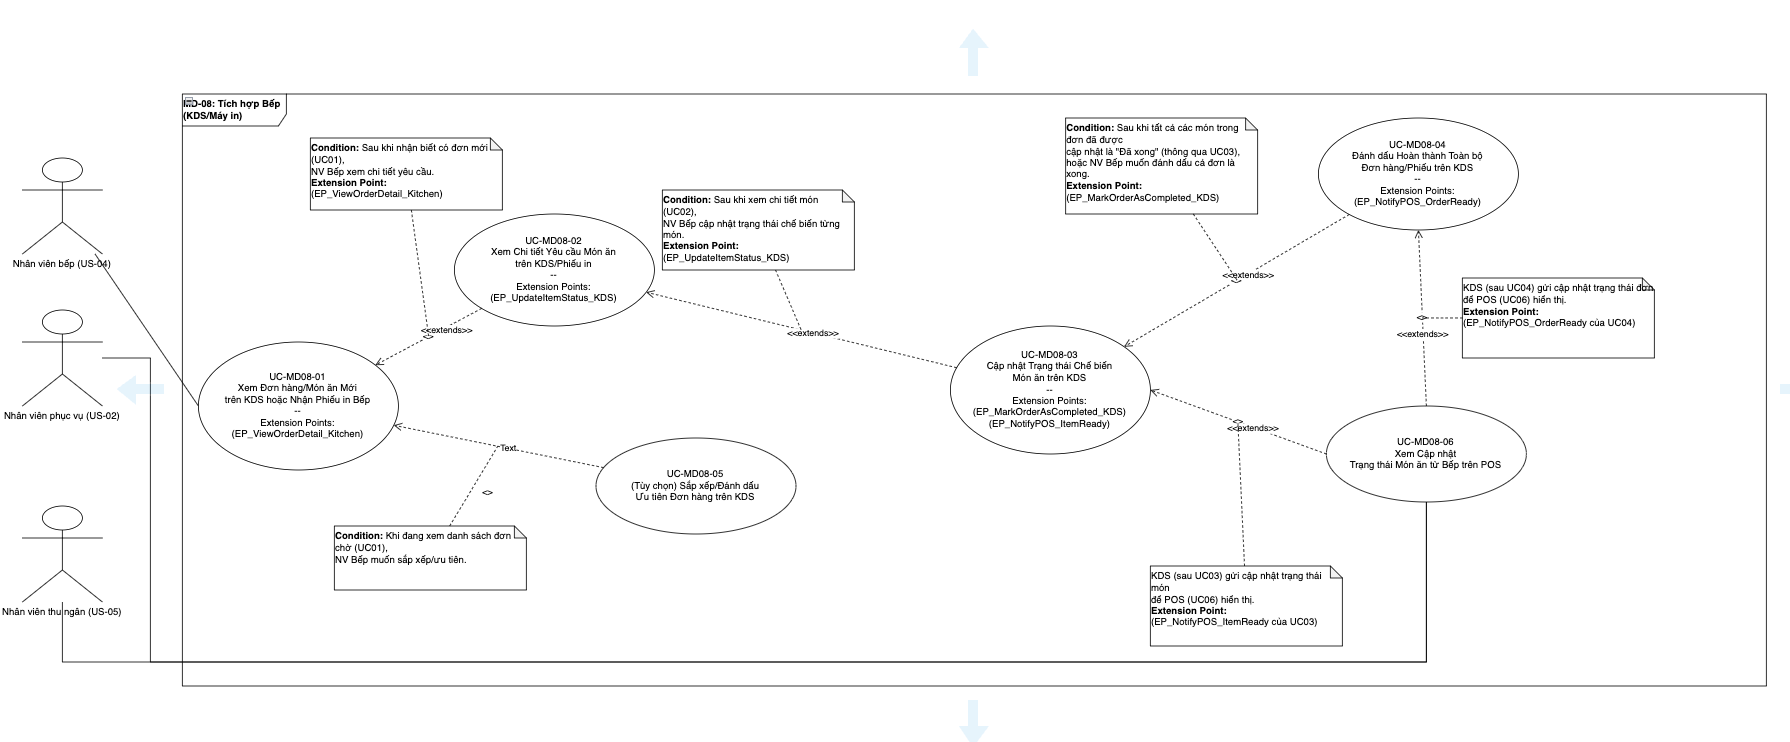
\includegraphics[width=15cm]{Sections/tong_quan/functional_spec/img/uc8.png}
    \vspace{0.5cm}
    \caption{Use case diagram cho Module MD-08}
    \label{fig:my_label}
\end{figure}

\begin{longtable}{|m{2cm}|m{2.5cm}|m{2.5cm}|m{4.5cm}|m{4cm}|}
\caption{Danh sách Yêu cầu Chức năng cho Module MD-08: Tích hợp Bếp (Kitchen Integration)} \label{tab:fr_md08_revised_v2} \\
\hline
\textbf{Mã Module} & \textbf{Mã Yêu cầu CN} & \textbf{Mã Người dùng} & \textbf{Tên Chức năng} & \textbf{Mô tả Ngắn} \\
\hline
\endhead % Header cho các trang tiếp theo
\hline
\endfoot % Footer cho bảng
\hline
\endlastfoot % Footer cho trang cuối cùng

MD-08 & FR-MD08-01 & US-04 & Xem Đơn hàng/Món ăn Mới trên KDS/Máy in Bếp & Nhân viên bếp xem các đơn hàng/món ăn mới được gửi đến KDS hoặc nhận phiếu in từ máy in bếp. (Việc gửi đi là kết quả của FR-MD05-08, FR-MD06-06, FR-MD07-06). \\
\hline
MD-08 & FR-MD08-02 & US-04 & Xem Chi tiết Yêu cầu Món ăn trên KDS/Phiếu in & Nhân viên bếp đọc thông tin chi tiết của từng món cần chuẩn bị: tên, số lượng, biến thể, ghi chú đặc biệt. \\
\hline
MD-08 & FR-MD08-03 & US-04 & Cập nhật Trạng thái Chế biến Món ăn trên KDS & Nhân viên bếp tương tác với KDS để đánh dấu trạng thái chế biến của món ăn (ví dụ: Bắt đầu làm, Đã xong). \\
\hline
MD-08 & FR-MD08-04 & US-04 & Đánh dấu Hoàn thành Toàn bộ Đơn hàng/Phiếu trên KDS & Nhân viên bếp đánh dấu toàn bộ các món trong một đơn hàng/phiếu đã được chuẩn bị xong trên KDS. \\
\hline
MD-08 & FR-MD08-05 & US-04 & Sắp xếp/Đánh dấu Ưu tiên Đơn hàng trên KDS & Nhân viên bếp thay đổi thứ tự hoặc đánh dấu ưu tiên cho các đơn hàng/phiếu trên KDS. \\
\hline
MD-08 & FR-MD08-06 & US-02/US-05 & Xem Cập nhật Trạng thái Món ăn từ Bếp trên POS & Nhân viên phục vụ/thu ngân xem được thông tin món nào đã sẵn sàng từ bếp (nếu KDS có gửi cập nhật về POS). \\
\hline

\end{longtable}


\subsubsubsection{Mục tiêu và Phạm vi}
\label{sssec:md08_objectives_scope}
Mục tiêu chính của module MD-08 là:
\begin{itemize}
    \item \textbf{Truyền tải chính xác yêu cầu món ăn:} Đảm bảo mọi chi tiết của đơn hàng (tên món, số lượng, biến thể, ghi chú đặc biệt) được gửi từ POS đến bếp một cách đầy đủ và không sai sót.
    \item \textbf{Tối ưu hóa quy trình làm việc trong bếp:} Giúp nhân viên bếp dễ dàng tiếp nhận, xem, quản lý và theo dõi tiến độ chuẩn bị các món ăn.
    \item \textbf{Giảm thiểu sai sót và nhầm lẫn:} Hạn chế việc trao đổi thông tin bằng miệng hoặc giấy tờ dễ thất lạc, từ đó giảm lỗi trong quá trình chế biến.
    \item \textbf{Cải thiện thời gian phục vụ:} Giúp bếp nhận yêu cầu nhanh hơn và quản lý thứ tự ưu tiên hiệu quả hơn (đặc biệt với KDS).
    \item \textbf{(Nếu dùng KDS) Cung cấp khả năng theo dõi và cập nhật trạng thái:} Cho phép nhân viên bếp đánh dấu trạng thái chế biến (đang làm, đã xong) và (tùy chọn) đồng bộ thông tin này ngược lại cho nhân viên phục vụ.
    \item \textbf{Hỗ trợ định tuyến thông minh:} Đảm bảo các món ăn được gửi đến đúng trạm chuẩn bị (ví dụ: món chính gửi bếp chính, đồ uống gửi quầy bar) nếu nhà hàng có nhiều khu vực bếp/bar.
\end{itemize}
Phạm vi của module bao gồm việc tiếp nhận yêu cầu món ăn từ hệ thống POS (MD-05, MD-06, MD-07), hiển thị thông tin chi tiết cho nhân viên bếp, và (nếu sử dụng KDS) cho phép nhân viên bếp tương tác để cập nhật trạng thái chế biến. Nó không bao gồm việc quản lý công thức, định lượng nguyên vật liệu, hay các chức năng quản lý kho chi tiết (thuộc các module khác).

\subsubsubsection{Đối tượng Sử dụng Chính}
\label{sssec:md08_primary_users}
Đối tượng người dùng chính của module này là:
\begin{itemize}
    \item \textbf{US-04 (Nhân viên bếp):} Là người trực tiếp sử dụng KDS hoặc nhận phiếu in từ máy in bếp để xem yêu cầu, chuẩn bị món ăn, và (nếu có KDS) cập nhật trạng thái chế biến.
\end{itemize}
Các đối tượng khác tương tác gián tiếp:
\begin{itemize}
    \item \textbf{US-02 (Nhân viên phục vụ) / US-05 (Nhân viên thu ngân):} Là người gửi yêu cầu chuẩn bị món từ POS. Họ cũng có thể (tùy chọn) nhận được cập nhật trạng thái món ăn từ KDS (UC-MD08-06).
    \item \textbf{US-01 (Quản lý nhà hàng) / US-10 (Quản trị viên Hệ thống):} Chịu trách nhiệm cấu hình máy in bếp, KDS, và các quy tắc định tuyến.
\end{itemize}

\subsubsubsection{Các Chức năng Chính}
\label{sssec:md08_key_functionalities}
Module MD-08 cung cấp các chức năng thiết yếu cho việc vận hành bếp, được mô tả chi tiết qua các Use Case sau:

\begin{itemize}
    \item \textbf{Tiếp nhận và Hiển thị Yêu cầu (UC-MD08-01, UC-MD08-02):}
    \begin{itemize}
        \item Nhân viên bếp xem các đơn hàng/món ăn mới xuất hiện trên Màn hình Hiển thị Bếp (KDS) hoặc nhận phiếu yêu cầu được in ra từ máy in bếp (UC-MD08-01).
        \item Nhân viên bếp xem thông tin chi tiết của từng yêu cầu món ăn, bao gồm tên món, số lượng, các tùy chọn biến thể và ghi chú đặc biệt (UC-MD08-02).
    \end{itemize}

    \item \textbf{Quản lý Trạng thái Chế biến trên KDS (UC-MD08-03, UC-MD08-04):} (Áp dụng nếu sử dụng KDS)
    \begin{itemize}
        \item Nhân viên bếp cập nhật trạng thái chế biến của từng món ăn cụ thể trên KDS (ví dụ: "Đang làm", "Đã xong") (UC-MD08-03).
        \item Nhân viên bếp đánh dấu hoàn thành toàn bộ một đơn hàng/phiếu trên KDS khi tất cả các món trong đó đã được chuẩn bị xong (UC-MD08-04).
    \end{itemize}

    \item \textbf{Tối ưu hóa và Đồng bộ hóa (UC-MD08-05, UC-MD08-06):} (Chủ yếu áp dụng cho KDS)
    \begin{itemize}
        \item (Tùy chọn) Nhân viên bếp có thể sắp xếp lại thứ tự hoặc đánh dấu ưu tiên cho các đơn hàng/phiếu trên KDS để quản lý công việc hiệu quả hơn (UC-MD08-05).
        \item (Tùy chọn) Hệ thống cho phép nhân viên phục vụ trên POS xem được thông tin cập nhật về trạng thái món ăn ("Đã xong") từ KDS (UC-MD08-06).
    \end{itemize}
\end{itemize}

\subsubsubsection{Tóm tắt Luồng Hoạt động Tổng thể}
\label{sssec:md08_overall_workflow}
Luồng hoạt động chính trong module Tích hợp Bếp thường diễn ra như sau:
\begin{enumerate}
    \item \textbf{Nhận yêu cầu từ POS:}
        \begin{itemize}
            \item Khi nhân viên phục vụ gửi yêu cầu chuẩn bị món từ POS (UC-MD05-08, UC-MD06-06, UC-MD07-06), thông tin được chuyển đến bếp.
            \item Nhân viên bếp Xem Đơn hàng/Món ăn Mới trên KDS hoặc Nhận Phiếu in Bếp (UC-MD08-01).
        \end{itemize}
    \item \textbf{Xem chi tiết và chuẩn bị:}
        \begin{itemize}
            \item Nhân viên bếp Xem Chi tiết Yêu cầu Món ăn trên KDS/Phiếu in (UC-MD08-02) để nắm rõ các yêu cầu về món, biến thể, và ghi chú.
            \item Nhân viên bếp tiến hành chuẩn bị món ăn.
        \end{itemize}
    \item \textbf{Cập nhật trạng thái (Nếu dùng KDS):}
        \begin{itemize}
            \item Trong quá trình chuẩn bị, nhân viên bếp Cập nhật Trạng thái Chế biến Món ăn trên KDS (UC-MD08-03), ví dụ: chuyển từ "Chờ" sang "Đang làm".
            \item (Tùy chọn) Nhân viên bếp có thể Sắp xếp/Đánh dấu Ưu tiên Đơn hàng trên KDS (UC-MD08-05) nếu cần.
            \item Khi tất cả các món trong một đơn/phiếu đã xong, nhân viên bếp Đánh dấu Hoàn thành Toàn bộ Đơn hàng/Phiếu trên KDS (UC-MD08-04).
        \end{itemize}
    \item \textbf{(Tùy chọn) Đồng bộ về POS (Nếu dùng KDS và có cấu hình):}
        \begin{itemize}
            \item Hệ thống cho phép nhân viên phục vụ Xem Cập nhật Trạng thái Món ăn từ Bếp trên POS (UC-MD08-06), giúp họ biết món nào đã sẵn sàng để phục vụ.
        \end{itemize}
\end{enumerate}
Module MD-08 giúp số hóa và tối ưu hóa giao tiếp giữa bộ phận phục vụ và bếp, góp phần nâng cao hiệu suất và chất lượng dịch vụ của nhà hàng.


